\section{Marco Teórico}


\subsection{Representación temporal y frecuencial de señales}
Fundamentalmente, el audio esta compuesto por formas de ondas. Cuando un objeto vibra genera ondas de presión que cuando alcanzan nuestros oídos son percibidas como sonido \cite{ritmo}. Si bien entonces podemos definir a una señal de audio como una variación continua, para su análisis digital nos interesa estudiar este tipo de señales en un dominio discreto. Para lograrlo, se toman muestras equiespaciadas de la señal continua, en un proceso que se denomina muestreo. La distancia temporal entre dos muestras contiguas es determinado según la frecuencia máxima que se desea representar, acorde al teorema de Nyquist \cite{openheim}. Entonces, una señal continua $x_{a}(t)$ que es muestreada a una frecuencia de $f_{s} = 1 / T_{s}$ muestras por segundo, produce la señal discreta $x(n)$ que se puede definir a partir dela señal continua a partir de la ecuación \ref{eqn:discreta}, que equivale a la representación vectorial vista en la ecuación   \ref{eqn:vector}, siendo $N$ el número de muestras tomadas. 

\begin{equation}
\label{eqn:discreta}
	x(n) = x_{a}(nT_{s})
\end{equation} 

\begin{equation}
\label{eqn:vector}
	x_{n} = [x(0), x(1),..., x(N-1) ]^{T}
\end{equation} 


Partiendo de esta representación temporal de la señal, se puede obtener una representación frecuencial de la misma a partir de la Transformada Discreta de Fourier (DFT) \cite{openheim} que matemáticamente equivale a la expresión \ref{eqn:furier1}, lo cual es útil para poder realizar un análisis mas profundo de la señal. La DFT permite entonces representar a la señal a partir de componentes frecuenciales complejas. Es decir que para cada punto se tiene un valor de amplitud y un valor de fase. A su vez, esta transformación supone un proceso reversible, por lo cual la señal temporal puede ser recuperada partiendo de la señal frecuencial, aplicando la expresión \ref{eqn:furier2}. 

\begin{equation}
\label{eqn:furier1}
	X[k] = \sum_{n=0}^{N-1} x[n]e^{-jnk2\pi/N} \qquad  0\leq k \leq N-1
\end{equation} 

\begin{equation}
\label{eqn:furier2}
	x[n] = {1}/{N}\sum_{k=0}^{N-1} X[k]e^{jnk2\pi/N} \qquad  0\leq n \leq N-1
\end{equation} 

El cálculo de esta transformación es costoso en términos computacinoales, y hay un alto grado de redundancia en este proceso. Por esto, comúnmente se utiliza una implementación definida como transformada rápida de Fourier que permite optimizar el cómputo de esta transformación \cite{fft}. 

Cuando se trabaja con señales no estacionarias es de interés evaluar la variación del espectro de frecuencias en el tiempo. Para esto se utiliza una transformación denominada transformada de Fourier de corto plazo (STFT por sus siglas en inglés) la cual consiste en una representación tridimensional formada al calcular la transformada de Fourier para sub-intervalos temporales de la señal, y luego representarlos de manera contigua \cite{ritmo}. De esta manera se obtiene un gráfico con dimensiones de tiempo, frecuencia y amplitud en donde se puede ver la evolución del espectro en función del tiempo. Un ejemplo de un espectrograma donde se conserva solo la magnitud se puede ver en la Figura \ref{fig:STFT}. 
 
 \begin{figure}[H]
  \centering{}
  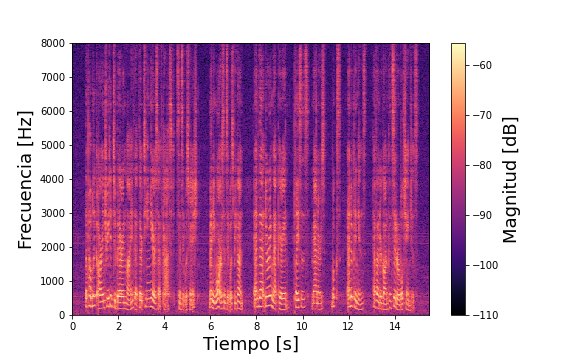
\includegraphics[scale=0.5]{STFT.png}
  \caption{Espectrograma de una señal de audio}
  \label{fig:STFT}
\end{figure}


\subsection{Respuesta al impulso y reverberación}

Si en un recinto se tiene una fuente y un micrófono captando a una cierta distancia de la fuente, las ondas sonoras que emite la fuente se reflejarán en las paredes del recinto y alcanzarán el micrófono inmediatamente después que la onda sonora directa. Las reflexiones continúan ocurriendo, y cada instancia de reflexión supone una disminución de la energía sonora de la onda, principalmente causada por el efecto de absorción acústica de las superficies que producen las reflexiones. En un determinado tiempo, la energía sonora decaerá en todo el recinto hasta ubicarse por debajo del ruido de fondo. A este proceso se lo denomina reverberación. Al camino mas corto entre la fuente y el punto de captura se denomina camino directo, y a la relación de nivel entre la presión sonora que genera la onda propia del camino directo y la presión que genera el efecto de reverberación se lo conoce como relación directo-reverberado. 

Si el micrófono se ubica cerca de la fuente va a captar en mayor medida la señal correspondiente al camino directo, y una pequeña porción del sonido reverberado. Es decir, una relación directo-reverberado alta. A medida que el punto de captura se aleja de la fuente va a captar una menor cantidad del sonido correspondientemente al camino directo, mientras que el campo reverberado se mantendrá aproximadamente invariante. Esto se traduce en una disminución de la relación directo-reverberado. 

De esta manera, habrá una distancia específica para la cual el nivel de presión sonora generado por la fuente sera igual al nivel de presión sonora generado por el efecto de la reverberación. Esta distancia se conoce como distancia crítica. Esta depende tanto de las condiciones del recinto como de las características del micrófono. 

La función de transferencia entre la fuente emisora y el micrófono se define como la respuesta al impulso del recinto y usualmente se denota como $h(t)$. Este será diferente para cualquier punto en el espacio dentro del recinto. Haciendo un análisis temporal de una respuesta al impulso, podemos identificar 3 partes: en primer lugar el nivel de sonido directo (producido por la onda que viaja a través de camino directo), las reflexiones tempranas (cuyo limite temporal vendrá definido por las características propias de cada recinto) y por último la cola reverberante. Esto se ve representado en la Figura \ref{fig:rir}. Se puede distinguir la parte de reflexiones tempranas y la cola reverberante partiendo de la suposición de que las reflexiones tempranas ocurren en un proceso determinístico, siendo altamente sensibles a pequeños cambios en la geometría del recinto, mientras que la cola reverberante es mas bien un proceso estocástico, y al depender de un mayor número de reflexiones no varia drásticamente frente a pequeños cambios de geometría. Analíticamente, la parte temprana y tardia de una respuesta al impulso se define segun las ecuaciones \ref{eqn:early} y \ref{eqn:late} respectivamente.

\begin{equation}\label{eqn:early}
h_{e}(t) = \left\{\begin{matrix}
h(t) & t_{d}-t_{0}\leq t \leq t_{d}+t_{0}\\ 
0 & e.o.c 
\end{matrix}\right.
\end{equation} 

\begin{equation}\label{eqn:late}
h_{l}(t) = \left\{\begin{matrix}
h(t) & t < t_{d} - t_{0} \\ 
h(t) & t > t_{d} + t_{0}\\ 
0 & e.o.c. 
\end{matrix}\right.
\end{equation} 

En donde, $h(t)$ corresponde a la respuesta al impulso, $h_{e}(t)$ corresponde a la parte temprana, $h_{l}(t)$ corresponde a la parte tardia, $t_{d}$ es el tiempo de retardo del camino directo y $t_{0}$ es el parámetro que define el largo temporal de la ventana de tolerancia. Comúnmente se utiliza un valor de $t_{0} = 2.5 ms$.

\begin{figure}[H]
  \centering{}
  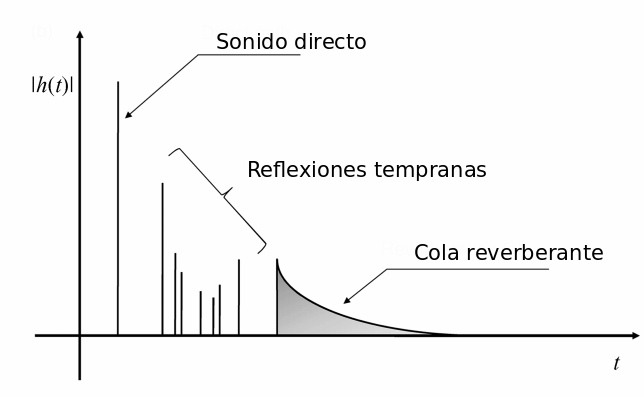
\includegraphics[scale=0.5]{rir.png}
  \caption{Secciones temporales de una respuesta al impuulso}
  \label{fig:rir}
\end{figure}

Idealmente, el micrófono captura una señal que corresponde a la convolución entre la respuesta al impulso del recinto y la señal fuente, como se ve en la ecuación \ref{eqn:impulso}. Esto equivale a una multiplicación en el dominio de la frecuencia de acuerdo con la transformada de Fourier, como se ve en la ecuación \ref{eqn:frecuencia}.  


\begin{equation}
\label{eqn:impulso}
	x(t) = h(t) * s(t)
\end{equation} 

\begin{equation}
\label{eqn:frecuencia}
	X(f) = H(f)S(f)
\end{equation} 

De esta manera se puede ver que la respuesta al impulso conserva toda la información sobre la influencia de la reverberación del recinto sobre la señal captada por el micrófono. 

\subsubsection{Relación directo-reverberado}

Es un descriptor acústico que se aplica sobre respuestas al impulso. Se define según la ecuación \ref{eqn:DRR} en la cual $h(n)$ representa la respuesta al impulso discreta obtenida. Los índices desde cero hasta $n_{d}$ representan las muestras correspondientes a la trayectoria directa, y las muestras que continúan luego de $n_{d}$ representan solo la reverberación producida por las trayectorias reflejadas. 

\begin{equation}
\label{eqn:DRR}
	DRR  [dB]= 10 Log_{10}(\frac{\sum_{n=0}^{n_d}h^{2}(n)}{\sum_{n=n_{d}+1}^{\infty}h^{2}(n)}) 
\end{equation}

Este parámetro es dependiente de la distancia entre el punto emisor y receptor, y del tiempo de reverberación del recinto. Realizando un análisis energético \cite{libro_dereverb} se puede obtener una expresión equivalente para este descriptor, la cual se muestra en la ecuación \ref{eqn:DRR2}.

\begin{equation}
\label{eqn:DRR2}
	DRR [dB]= 10 Log_{10}(\frac{QR}{16 \pi D^{2}}) 
\end{equation}



Como esta definición inicialmente se piensa en un dominio continuo, la primera intuición es pensar que el camino directo está fielmente representado por la mayor magnitud en la parte temprana de la respuesta al impulso. Sin embargo, esto solo es correcto cuando el tiempo de propagación entre la fuente y el receptor es un múltiplo entero del período de muestreo. Por esto, trabajar con frecuencias de muestreo finitas (dominio discreto) en general deriva en que la representación del camino directo se produzca a través de una función seno cardinal ($Sinc$) correspondiente a la ventana de muestreo, centrada de acuerdo al retardo correspondiente al tiempo de propagación. En cambio, cuando se trata de respuestas al impulso sintéticas, el camino directo puede ser computado de forma separada del resto. Es decir, se puede determinar con exactitud el aporte del campo directo y del campo reverberado, lo que permite el cálculo del parámetro $DRR$ con una mayor exactitud. 




\subsection{Inteligibilidad y parámetros de calidad de percepción}

Para caracterizar la señal del habla propagándose en condiciones reverberantes se utilizan métricas objetivas derivadas de la respuesta al impulso del recinto en cuestión, como por ejemplo el tiempo de reverberación o la relación energética entre la señal directa y el campo reverberado. En cambio, al considerar el proceso de dereverberación de estas señales las respuestas al impulso requieren ser estimadas, lo que usualmente conduce a una caracterización de baja calidad. Además, los algoritmos de dereverberación pueden introducir artefactos audibles a la señal voz, los cuales no son contemplados por las respuestas al impulso estimadas. Es por esto que es preciso utilizar métodos de medida de calidad basados en la señal dereverberada. Las pruebas subjetivas son el método más confiable para evaluar la calidad percibida de una señal de habla dereverberada. Sin embargo, este método es costoso y requiere mucho tiempo, por lo cual se vuelve inviable su aplicación para procesamientos en tiempo real. Para aplicaciones prácticas se definieron entonces métodos objetivos de medición de calidad basados en la señal dereverberada como reemplazo de las pruebas subjetivas. Estos métodos consisten en algoritmos que de manera objetiva y repetible buscan estimar la calidad percibida de la señal, por lo cual, un método resulta efectivo cuando logra obtener una alta correlación con las respuestas subjetivas. Estos métodos se clasifican en intrusivos o no intrusivos, dependiendo de si requieren o no una señal de referencia para realizar la estimación. Poder contar con una señal de referencia para realizar estas estimaciones es usualmente una dificultad, por lo cual se presta mayor interés en aquellos métodos no intrusivos. 

\subsubsection{Relación energía de modulación de voz a reverberación}

Este parámetro de medida de calidad para señales dereverberadas se basa en obtener características de la reverberación partiendo del espectro de modulación de la señal \cite{SRMR}. La formulación de este parámetro se basa en el hecho de que la cola reverberante de cualquier respuesta al impulso puede ser modelada como ruido blanco Gaussinano exponencialmente amortiguado. Esta característica puede ser explotada en el análisis del espectro de modulación de la señal bajo análisis para obtener descriptores del efecto de la reverberación.

\subsubsection{Inteligibilidad objetiva de corto termino extendida}
Este parámetro está basado en características extraídas a partir de la correlación de corto término entre la señal limpia y la señal procesada. Es aplicable para evaluar aquellos procesos que realizan transformaciones no lineales \cite{ESTOI}. Su funcionamiento se basa en aplicar una ventana de análisis de $384$ $ms$ en las envolventes de amplitud de las subbandas de la señal analizada. Estas ventanas temporales se aplican en pos de contemplar frecuencias de modulación que son relevantes para la inteligibilidad. En estos lapsos temporales se calculan coeficientes de correlación espectrales que son luego promediados. De esta manera, este parámetro puede ser interpretado en términos de una descomposición ortogonal de espectrogramas energéticamente normalizados que son luego ordenados de acuerdo a su contribución a la inteligibilidad estimada. 

\subsubsection{Relación señal a distorsión}

Este descriptor fue ampliamente utilizado en tareas de separación de fuentes y refuerzo de señales de habla. Esta basado en el cómputo de la relación señal a interferencia (SIR), y en la relación señal a artefacto (SAR) \cite{SAR}. En las tareas de dereverberación, estas medidas pueden ser interpretadas como proporcionales a la supresión de componentes reverberantes tardías e inversamente proporcionales a la distorsión en la señal del habla, respectivamente. Contemplando estos valores, el parámetro final contempla la calidad general de la señal dereverberada.  

\subsection{Redes neuronales y algoritmos de aprendizaje}

La base de los algoritmos de aprendizaje profundo se encuentra en la neurona artificial. Esta consiste en un modelo que parte de los principios de funcionamiento de las neuronas biológicas \cite{neurona}. El perceptrón \cite{perceptron} fue de las primeras arquitecturas formalmente implementadas y que se considera la unidad básica de  estos algoritmos. Un esquema de una neurona artificial básica se puede ver en la Figura \ref{fig:neurona}. Las componentes básicas de una neurona artificial son: 

\begin{itemize}
    \item \textbf{Entradas}: Recibe los datos que van a ser procesados en esta unidad.
    \item \textbf{Pesos sinápticos}: Parámetros de ponderación. Cada entrada se asocia a uno de estos parámetros. Es el valor que se va ajustando cuando el modelo se encuentra en la etapa de entrenamiento. En ellos se ve reflejado la propagación del error. 
    
    \item \textbf{Suma ponderada}: Los pesos sinápticos se asocian a cada entrada a partir de una regla de propagación que consiste en una suma ponderada.
    \item \textbf{Función de activación}: Función que se aplica a la salida de la suma ponderada, cuya salida representa la salida final de la unidad. Esta se determina de manera de poder agregar complejidad al modelo. Algunos ejemplos de funciones de activación se pueden ver en la figura \ref{fig:activación}. 
    
    \item \textbf{Salida}: Es el resultado de aplicar el proceso completo al conjunto de entradas. En una estructura, esta salida puede ser la entrada de una o varias unidades subsiguientes. 
\end{itemize}

\begin{figure}[H]
  \centering{}
  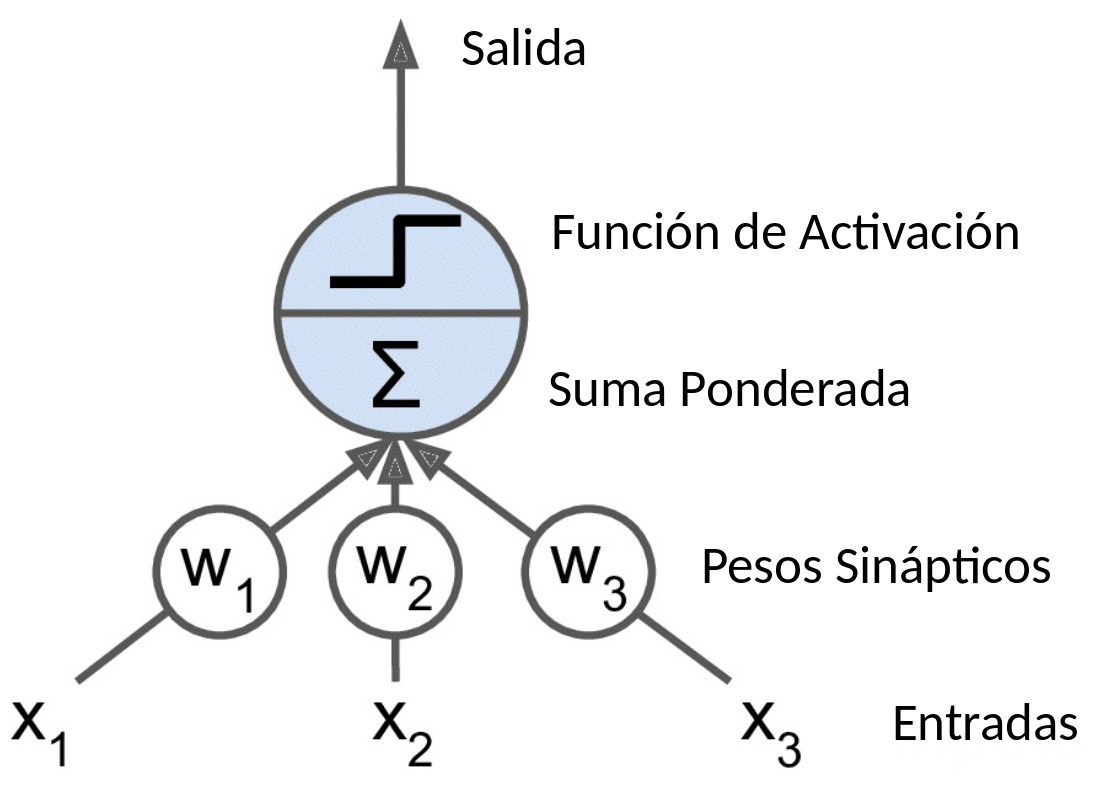
\includegraphics[scale=0.20]{neurona.png}
  \caption{Esquema de neurona artificial}
  \label{fig:neurona}
\end{figure}

\begin{figure}[H]
  \centering{}
  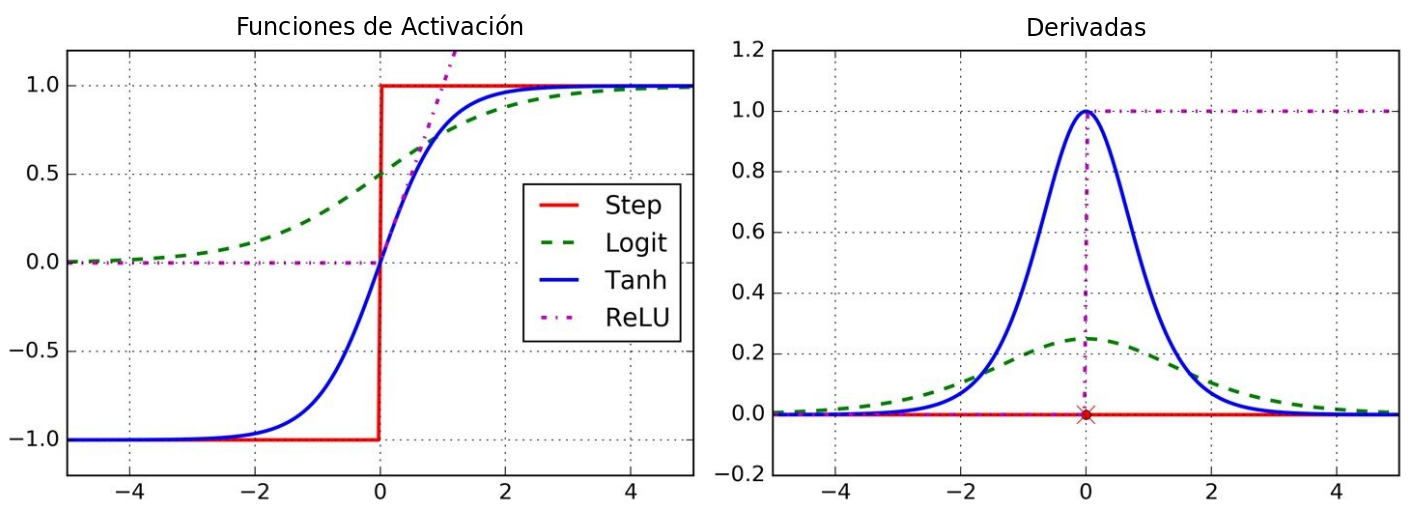
\includegraphics[scale=0.35]{activacion.png}
  \caption{Funciones de activación y sus derivadas}
  \label{fig:activación}
\end{figure}

\subsubsection{Modelos basados en redes neuronales}

Los modelos basados en redes neuronales son sistemas compuestos por capas que agrupan unidades computacionales (neuronas artificiales). En una capa, las entradas y salidas de las neuronas artificiales que la componen están agrupadas. Diferentes capas se relacionan formando sistemas de acuerdo al problema que se busque resolver. En general, un sistema se compone por una capa de entrada, una capa de salida, y un número finito de capas ocultas intermedias. De esta forma, el sistema recibe valores de entrada, los procesa a través de las distintas capas que componen la red, y otorga valores de salida. Un esquema de este funcionamiento se puede ver en la Figura \ref{fig:red}.

\begin{figure}[H]
  \centering{}
  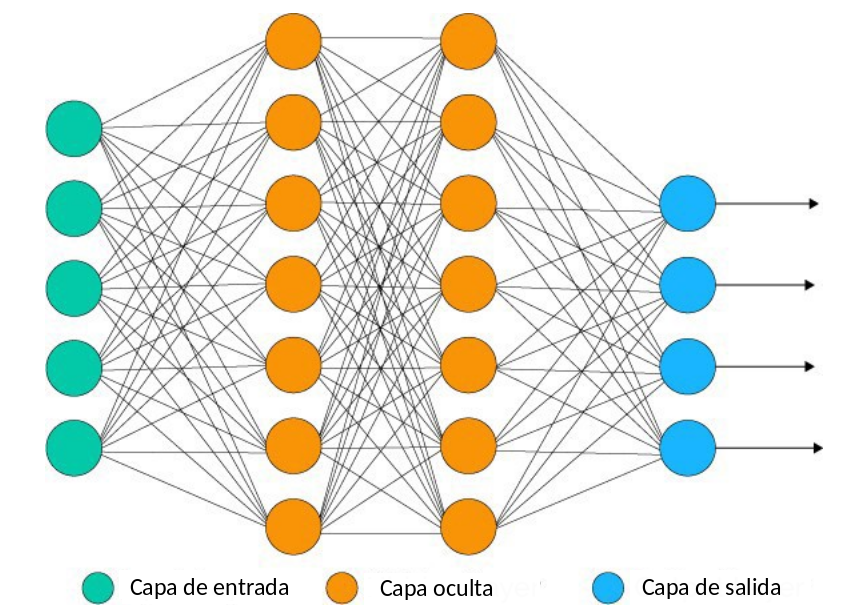
\includegraphics[scale=0.35]{red.png}
  \caption{Esquema básico de red neuronal}
  \label{fig:red}
\end{figure}

Catalogar a estos sistemas como de aprendizaje 'profundo' hace referencia al hecho de tener sucesivas capas de representación \cite{franchute}. Cuando un modelo se compone de un mayor numero de capas, se lo considera mas 'profundo'. 

Estas estructuras de redes neuronales aprenden automáticamente al ser expuestas a un conjunto de datos. El proceso de aprendizaje se puede pensar como la evaluación de un mapeo de valores de entrada a ciertos valores objetivos de salida. Esto es, se toman valores de entrada, se los transforman a lo largo de las capas que componen la red produciendo valores de salida, y se comparan estas salidas con los valores de salida objetivos. Entonces, la especificación del proceso que está siendo implementado por el sistema se encuentra reflejado en los pesos sinápticos de las neuronas que componen cada capa. El aprendizaje se obtiene a partir de poder modificar estos pesos sinápticos acorde a las diferencias que se obtengan entre las salidas producidas por la red y las salidas que se tienen como objetivo. Para lograr esto último, los algoritmos de redes neuronales utilizan determinadas funciones: 

\begin{itemize}
\item\textbf{Función de costo}: También denominada función objetivo, o función de pérdida. Recibe las salidas de la red y las salidas esperadas y evalúa que tanto difieren entre sí. Estas diferencias las traduce a una medida de distancia a partir de una expresión matemática que se define en función del problema que se busca resolver. Entonces, para cada estimación de la red, esta función otorga un puntaje que explica cuan lejos está el valor estimado del valor pretendido.  

\item\textbf{Función de optimización}: Esta función aplica el algoritmo de propagación del error hacia atrás, que es una parte fundamental de un algoritmo de aprendizaje profundo. Este cálculo permite estimar el aporte que tiene cada peso sináptico en el error final de la estimación de la red, y por lo tanto permite ajustar los valores de estos pesos sinápticos estratégicamente para conseguir minimizar la distancia computada por la función de costo. 

\end{itemize} 

Entonces, la salida de la función de costo se utiliza como realimentación del sistema a través de la función de optimización. De este modo, el entrenamiento consiste en un bucle en el cual en cada iteración el sistema evalúa una instancia de los datos de entrenamiento (valores de entrada y de salida), y ajusta los pesos sinápticos en pos de reducir el error calculado. Un esquema que expone este funcionamiento se ve en la Figura \ref{fig:esquema}. Repetir este ciclo un número suficiente de veces conduce a la convergencia del valor de error. 

\begin{figure}[H]
  \centering{}
  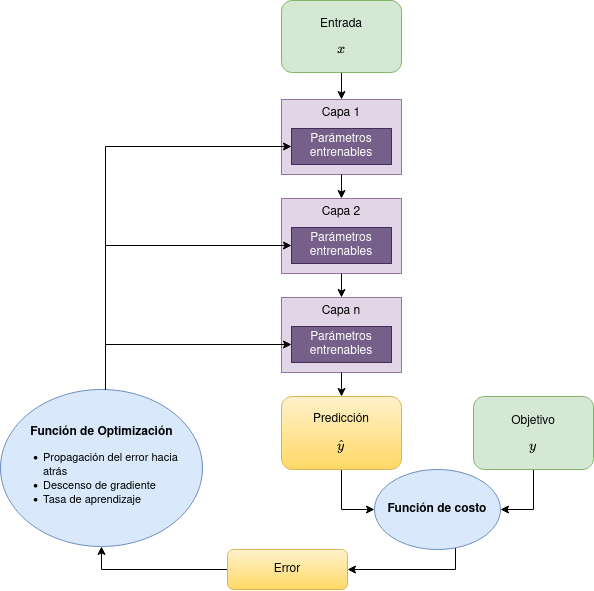
\includegraphics[scale=0.35]{esquema_red.png}
  \caption{Diagrama de flujo del bucle de entrenamiento de una sistema de red neuronal}
  \label{fig:esquema}
\end{figure}

Por último, la manera en que el sistema de red neuronal recibe y procesa los datos también influye en el desempeño de la misma. El objetivo final del sistema es alcanzar un grado de generalización que le permita procesar adecuadamente instancias de datos que no hayan sido reveladas ante la red en la etapa de entrenamiento. Por esto, el conjunto total de los datos se divide en tres subgrupos: 

\begin{itemize}
\item\textbf{Conjunto de entrenamiento}: Este conjunto de datos es el que se utiliza en la etapa de entrenamiento para optimizar los parámetros de la red. Aquí se concentra el mayor volumen de datos.

\item\textbf{Conjunto de validación}: Sobre este conjunto se mide el desempeño del sistema a lo largo de su entrenamiento. Los resultados obtenidos del procesamiento de este conjunto sirven para ajustar variables que requieren ser especificadas de manera previa al entrenamiento. Estos parámetros se denominan hiper parámetros.
 
\item\textbf{Conjunto de prueba}: Este conjunto es el que se utiliza para medir el rendimiento final del sistema. Como contiene instancias que no fueron utilizadas en las etapas de entrenamiento y ajuste de parámetros, el análisis del procesamiento de este conjunto sirve para medir el nivel de generalización que el sistema logró alcanzar. 

\end{itemize}


El conjunto de datos de entrenamiento se segmenta en lotes. En cada iteración de entrenamiento la red neuronal recibe un lote, lo procesa, aplica la función de costo y ajusta los pesos sinápticos de cada capa. Cuando la red procesó todos los lotes que componen el conjunto de datos de entrenamiento se dice que transcurrió una época. El proceso de entrenamiento depende en cierta medida del tamaño de los lotes \cite{franchute}. Si consideramos la curva de la función de costo de un parámetro como la de la Figura \ref{fig:costo_curva}, vemos que existen mínimos locales y mínimos globales a lo largo de la misma. En el proceso de entrenamiento se busca minimizar este valor de costo. Si se toman lotes muy pequeños, lo que se traduce en desplazamientos pequeños a lo largo de esta curva, se corre el riesgo de quedar confinado en un mínimo local. De igual manera, un conjunto demasiado grande produciría saltos demasiado grandes en comparación a las fluctuaciones de esta curva, haciendo que se obtengan valores de costo aleatorios. 

\begin{figure}[H]
  \centering{}
  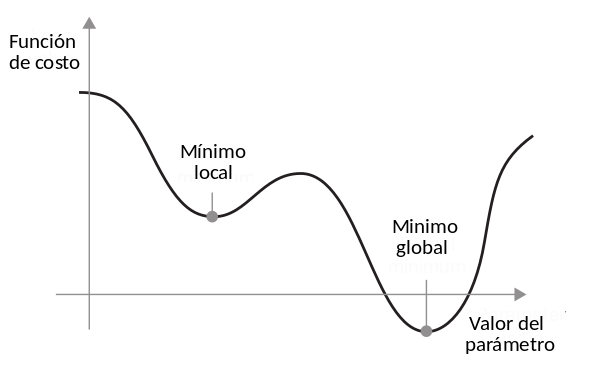
\includegraphics[scale=0.35]{costo_curva.png}
  \caption{Curva de costo para un parámetro}
  \label{fig:costo_curva}
\end{figure}

El orden en el que los datos son presentados ante el modelo puede influenciar positiva o negativamente en el resultado final del entrenamiento. Existen técnicas de optimización que se desarrollaron partiendo de cualidades propias del aprendizaje en seres humanos y anaimales, como el hecho de que el aprendizaje resulta mejor cuando las instancias de aprendizaje estan organizadas en un orden significativo, añadiendo gradualmente mayor cantidad de conceptos y por ende una mayor complejidad. Esta idea se traslada al entrenamiento de algoritmos de aprendizaje profundo con el desarrollo de una estrategia denominada aprendizaje por currículum \cite{cv}. La misma consiste en seleccionar cuales datos y en que orden presentarlos al sistema durante el aprendizaje, de manera de guiar el entrenamiento para que inicialmente se aprendan los conceptos mas sencillos del problema, e ir gradualmente aumentando el grado de complejidad de la tarea. El aprendizaje por curriculum se define como una estrategia de optimización global. Dependiento de la tarea sobre la que se aplica, puede lograr en menor o mayor medida que un sistema logre un mejor nivel de generalización asi como también llegar al punto de convergencia en un menor tiempo de entrenamiento.  


\subsubsection{Redes neuronales convolucionales}

Las redes neuronales convolucionales emergen del estudio de la corteza visual del cerebro. En los últimos años, estas estructuras fueron utilizadas para resolver tareas visuales complejas (análisis de imágenes). El componente principal es la capa convolucional. Para el análisis de imágenes, estas capas se concatenan de manera que la primera capa no contempla cada píxel de la imagen, sino que solo se enfoca un número acotado de píxeles que caen dentro de su campo perceptivo. De igual manera, las capas subsiguientes se enfocan en las salidas de un conjunto acotado de neuronas de la capa precedente. Este funcionamiento se ilustra en la Figura \ref{fig:convnet}. 

\begin{figure}[H]
  \centering{}
  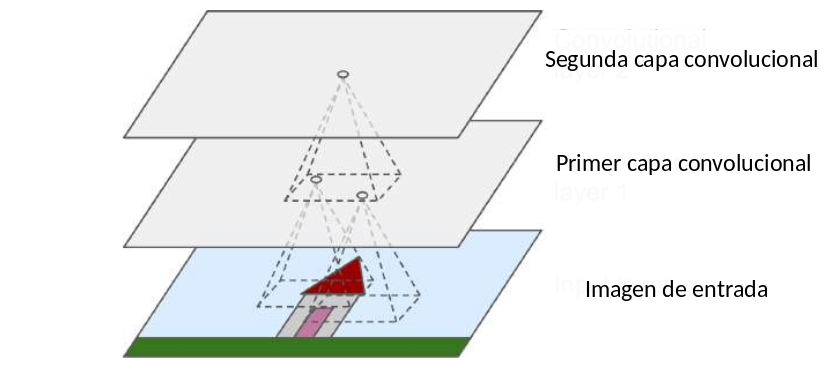
\includegraphics[scale=0.35]{convnet.png}
  \caption{Capas convolucionales con campos receptivos locales rectangulares}
  \label{fig:convnet}
\end{figure}

Formar esta estructura le permite a la red aprender diferentes patrones estructurales locales de manera jerárquica \cite{lagartija}. Estas capas se distinguen por dos propiedades fundamentales: 

\begin{itemize}
\item Los patrones que se aprenden son invariantes al desplazamiento. Esto quiere decir, que si se aprende de un patrón ubicado en un lugar específico de una imagen, este mismo patrón puede ser identificado en cualquier otra ubicación dentro de la imagen. 

\item Cuando estas capas se concatenan formando redes logran aprender jerarquías espaciales de patrones. Esto les permite aprender de manera eficiente conceptos visuales cada vez más complejos y abstractos. 
\end{itemize}

\begin{figure}[H]
  \centering{}
  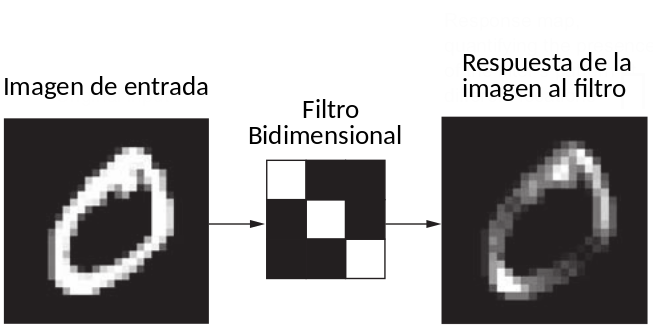
\includegraphics[scale=0.35]{filtro.png}
  \caption{Representación de la aplicación de un filtro bidimensional sobre una imagen}
  \label{fig:numerito}
\end{figure}

El procesamiento que ocurre en una capa convolucional consiste en la aplicación de uno o varios filtros bidimensionales sobre la imagen de entrada, lo cual genera mapas de respuestas que representan la presencia del patrón del filtro a lo largo de la imagen, como se puede apreciar en la Figura \ref{fig:numerito}. En este tipo de capas, el aprendizaje se traduce en determinar la forma de los filtros que se deben aplicar para conseguir los resultados esperados. Teniendo en cuenta este proceso, las variables que se deben definir en cada capa son: 

\begin{itemize}
\item\textbf{Tamaño del filtro}: Define el tamaño del campo perceptivo de cada unidad de procesamiento de la capa. Valores comunes son $3x3$ o $5x5$. En la Figura \ref{fig:variables_conv} se ve un ejemplo de un filtro de tamaño $3x3$.

\item\textbf{Tamaño del salto}: Determina la distancia horizontal y vertical entre campos perceptivos de dos unidades contiguas. Hacer que este valor sea mayor a uno permite reducir las dimensiones de la imagen de entrada al atravesar la capa convolucional. Esto se puede apreciar en la Figura \ref{fig:variables_conv} en donde se aplica un tamaño de salto igual a dos (tanto en sentido vertical como horizontal). 

\item\textbf{Relleno de ceros}: Cuando se pretende mantener invariables las dimensiones de entrada y salida de una capa convolucional, se suele aplicar un relleno con ceros en los contornos de la imagen. La cantidad de ceros agregados dependerá de las características del filtro a aplicar. Aplicar un relleno de ceros produce un fenómeno denominado efecto de borde \cite{lagartija}. 

\item\textbf{Cantidad de filtros aplicados}: El número de filtros computados por la convolución. 

\end{itemize}

\begin{figure}[H]
  \centering{}
  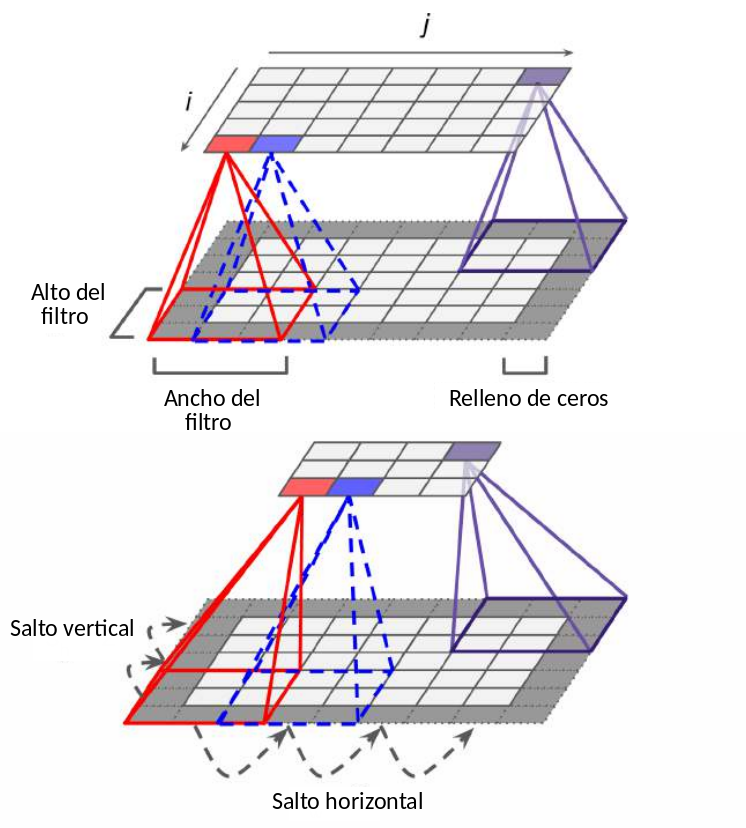
\includegraphics[scale=0.35]{filtrosconv.png}
  \caption{Parámetros de procesamiento en capas convolucionales}
  \label{fig:variables_conv}
\end{figure}

De esta manera, las capas convolucionales permiten construir modelos con menos cantidad de parámetros a entrenar, distribuidos adecuadamente para conseguir la generalización de conceptos visuales complejos. 

\subsection{Curriculum Learning}


\subsection{Dereverberación por filtrado temporal-frecuencial}

\subsubsection{Máscaras de amplitud}

Entre los numerosos métodos estudiados para abordar la tarea de la dereverberación, en la actualidad el análisis del espectro temporal-frecuencial ha tomado una importancia central debido a la posibilidad de explotar este enfoque utilizando herramientas como redes neuronales convolucionales y otros algoritmos de aprendizaje profundo. Partiendo de una señal con reverberación, se extrae una representación en tiempo-frecuencia a partir de transformaciones como la transformada de corto término de Fourier (STFT). Una vez obtenido este espectrograma, lo que se busca es descifrar el proceso necesario para obtener un nuevo espectro que se corresponda con la señal anecoica (descartando el efecto de la reverberación). Entonces, el proceso de dereverberación se puede resumir a la estimación de un filtro variable con el tiempo que se aplica sobre el espectrograma con reverberación. Estudios previos demostraron que la fase no aporta información significativa para estas tareas \cite{fase1}\cite{fase2}, por lo cual se pueden realizar estos procesos únicamente sobre la magnitud de los espectrogramas, descartando la información de fase. Considerando esto, el proceso de dereverberación se reduce a la expresión de la ecuación \ref{eqn:dereverb}, en donde $STFT_{Y}$ es el espectrograma de amplitud la señal anecoica, $STFT_{X}$ es el espectrograma de amplitud de la señal con reverberación y $M$ es la máscara ideal que representa el filtrado en el dominio tiempo-frecuencia. En otras palabras, el espectro de amplitud de la señal dereverberada se obtiene aplicando la máscara ideal sobre el espectro de amplitud con reverberación. 
 
\begin{equation}
\label{eqn:dereverb}
	STFT_{Y}(t,f)= M(t,f) STFT_{X}(t,f) 
\end{equation}

\begin{equation}
\label{eqn:dereverb2}
	M(t,f) =  \frac{STFT_{Y}(t,f)}{STFT_{X}(t,f)} 
\end{equation}

Por otro lado, de la ecuación \ref{eqn:dereverb2} se puede inferir que la mascara ideal puede tomar valores en el dominio $[-\infty , +\infty]$. Esto puede ser un contraproducente para la utilización de algoritmos de aprendizaje supervisado, donde lo conveniente es trabajar con instancias acotadas en un rango de valores del dominio $[-1 , +1]$. Para conseguir cambiar el dominio de las máscaras se realiza una compresión de los valores a través de una función tangencial hiperbólica. La misma se expresa en la ecuación \ref{eqn:compresion}, en donde $M^{'}(t,f)$ corresponde a la máscara comprimida. Luego de aplicar esta transformación, el dominio resultante pasa a ser $[-Q , +Q]$. El parámetro $C$ controla la pendiente de la tangente hiperbólica. 

\begin{equation}
\label{eqn:compresion}
	M^{'}(t,f) = Q\frac{1-e^{CM(t,f)}}{1+e^{CM(t,f)}}  
\end{equation}

De igual manera, partiendo de una máscara comprimida se puede recuperar la máscara original a través de la ecuación \ref{eqn:descompresion}. 

\begin{equation}
\label{eqn:descompresion}
	M(t,f) = \frac{-1}{C}log(\frac{Q-M^{'}(t,f)}{Q+M^{'}(t,f)})
\end{equation}

\subsubsection{Sintesis de audio a partir de espectrogramas}

Para realizar procesamiento de audio a partir de modificar espectros temporales-frecuenciales es necesario poder pasar de información de audio temporal a un dominio temporal-frecuencial (utilizando una transformación como la transformada de corto término de Fourier) y también poder recuperar información de audio partiendo de un espectrograma que ha sido modifcado. Esto último puede ser un problema, porque ciertos procesos pueden generar espectrogramas que no sean consistentes, es decir, que no haya ninguna señal en el dominio temporal que se condiga con el espectrograma generado. Para solucionar esta cuestión se desarrollaron algoritmos que buscan estimar una señal temporal cuyo espectrograma sea el mas cercano posible al espectrograma que se quiere antitransformar. Este es el caso del algoritmo propuesto por Griffin et. al. \cite{griffinlim}. El algoritmo consiste en un bucle iterativo que busca minimizar el error cuadrático medio entre la señal estimada y el espectrograma modificado. En la figura \ref{fig:griffin} se muestra un diagrama de bloques que explica el funcionamiento básico del algoritmo. 

\begin{figure}[H]
  \centering{}
  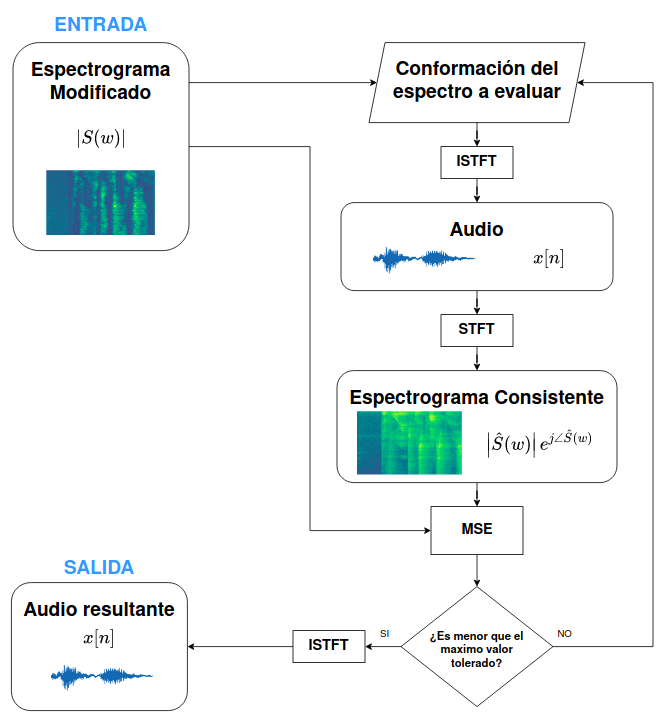
\includegraphics[scale=0.40]{griffin.png}
  \caption{Diagrama en bloques del algoritmo de Griffin-Lim.}
  \label{fig:griffin}
\end{figure}

El espectrograma de entrada $\left | S(w) \right |$ inicialmente se combina con una fase aleatoria para formar un espectrograma complejo. Este se antitransforma obteniendo una señal de audio, la cual vuelve a ser transformada obteniendose un nuevo espectrograma complejo $\left | \hat{S}(w) \right |e^{j\angle \hat{S}(w)}$. Este espectrograma es consistente, pues deriva de la transformación de una señal de audio real. Se puede probar que combinar esta fase resultante $\angle \hat{S}(w)$ con el espectrograma modificado de entrada $\left | S(w) \right |$ disminuye el error cuadrático entre los espectrogramas evaluados (es decir, entre el espectrograma consistente y el inconsistente). De esta manera, este proceso se repite hasta lograr que el error cuadratico medio descienda hasta un cierto valor deseado. Cuando esta condición se cumple, el espectrograma complejo que causa esta condición se antitransforma generando la señal de audio resultante final. 

